\documentclass[11pt]{article}
\usepackage[margin=1in]{geometry}
\usepackage{mathpazo}
\usepackage{amsmath,amssymb}
\usepackage{microtype}
\usepackage{booktabs}
\usepackage{graphicx}
\usepackage[dvipsnames]{xcolor}
\usepackage{tikz}
\usetikzlibrary{positioning,arrows.meta,calc,fit,backgrounds}
\usepackage[most]{tcolorbox}
\usepackage{enumitem}
\usepackage{listings}
\usepackage[font=small,labelfont=bf]{caption}
\usepackage{hyperref}
\hypersetup{colorlinks=true,linkcolor=MidnightBlue,citecolor=MidnightBlue,urlcolor=MidnightBlue}
\usepackage{cleveref}
\urlstyle{tt}
\def\UrlBreaks{\do\_\do/\do.}
\newcommand{\file}[1]{\nolinkurl{#1}}
\newcommand{\code}[1]{\texttt{#1}}
\newcommand{\mhh}{m_{hh}}
\newcommand{\bw}{\boldsymbol{\omega}}
\newcommand{\bp}{\boldsymbol{p}}
\newcommand{\bx}{\boldsymbol{x}}
\newcommand{\data}{\mathcal{D}}

\definecolor{trainable}{HTML}{1B6CA8}
\definecolor{physics}{HTML}{2E933C}
\definecolor{datac}{HTML}{7B4EA3}
\definecolor{warn}{HTML}{C0392B}

\newtcolorbox{keyidea}[1][]{enhanced,breakable,colback=physics!6,colframe=physics!70!black,
  fonttitle=\bfseries,title={#1},boxrule=0.6pt,arc=2pt,left=6pt,right=6pt}
\newtcolorbox{aside}[1][]{enhanced,breakable,colback=trainable!5,colframe=trainable!70!black,
  fonttitle=\bfseries,title={#1},boxrule=0.6pt,arc=2pt,left=6pt,right=6pt}
\newtcolorbox{assume}[1][]{enhanced,breakable,colback=datac!5,colframe=datac!70!black,
  fonttitle=\bfseries,title={#1},boxrule=0.6pt,arc=2pt,left=6pt,right=6pt}
\newtcolorbox{watch}[1][]{enhanced,breakable,colback=warn!5,colframe=warn!70!black,
  fonttitle=\bfseries,title={#1},boxrule=0.6pt,arc=2pt,left=6pt,right=6pt}
\setlist{itemsep=2pt,topsep=3pt}
\setlength{\emergencystretch}{3em}

\lstset{language=Python, basicstyle=\ttfamily\small, columns=fullflexible,
  keepspaces=true, commentstyle=\color{physics!70!black}\itshape,
  keywordstyle=\color{trainable!90!black}\bfseries, stringstyle=\color{datac},
  showstringspaces=false, frame=single, rulecolor=\color{gray!40},
  backgroundcolor=\color{gray!3}, xleftmargin=4pt, xrightmargin=4pt,
  aboveskip=6pt, belowskip=6pt}

\title{\textbf{Where does the model error come from?}\\[4pt]
\large A benchmark without a network, residual diagnostics, and a plan\\[4pt]
\normalsize P.~Bhat, N.~De~Filippis, K.\,F.~Johnson, H.\,B.~Prosper, R.~Starnes}
\date{October 31, 2026}
\begin{document}
\maketitle

\begin{keyidea}[In brief]
\begin{enumerate}
  \item \textbf{The network is not the limitation.} A fit with 23 free numbers per $m_{hh}$
    bin and no network, the best any model of the form $\sigma = \sum_i C_i(\theta)a_i(m_{hh})$
    can do, matches the fine-tuned ensemble on the test spectra (median $\chi^2/N$ 1.088 vs
    1.085; 1.58 vs 1.65 per bin below 555~GeV). A better network cannot remove the model error.
  \item \textbf{The excess is in the agreement between POWHEG and the 23-term form.} It is
    not count statistics, not the $\chi^2$ definition, not the normalisation, and not the
    statistical uncertainty of the fit.
  \item \textbf{It grows with cancellation and is smooth in $m_{hh}$.} Spectra whose cross
    section is a small difference of large terms have $\langle z^2\rangle \approx 1.9$, and
    their residuals are correlated between neighbouring bins (0.56); spectra without
    cancellation agree with the 23-term form to within Poisson noise ($\langle z^2\rangle
    \approx 1.02$--1.08).
  \item \textbf{A better error model follows.} A discrepancy proportional to the size of the
    individual terms, $\varepsilon(m_{hh})\sum_i|C_ia_i|$, with $\varepsilon \approx
    0.1$--0.9\%, calibrates every degree of cancellation (0.97--1.06), where the current
    $a(m_{hh})\sigma_k^2$ under-covers the strongest-cancellation fifth (1.52).
  \item \textbf{The likely origin is the generator}, a small relative inaccuracy of each
    coupling component, for example from the interpolated two-loop virtual amplitudes.
    This is a question for the people who produced the samples.
\end{enumerate}
\end{keyidea}

\tableofcontents

% ===========================================================================
\section{A benchmark without a network}
\label{sec:free}

In bin $k$ of every spectrum, \texttt{HEFTNet} predicts $\sum_{i=1}^{23} C_i(\theta)\,a_i(m_k)$:
the cross section is \emph{linear} in the 23 numbers $a_i(m_k)$. So the best possible values
of those numbers, for this functional form and these data, follow from a weighted linear
least-squares fit in each bin separately, with no network, no smoothness and nothing shared
between bins:
\begin{equation}
  \hat{\boldsymbol a}_k = \arg\min_{\boldsymbol a} \sum_{s} \frac{\big(t_{sk} -
  \boldsymbol C(\theta_s)\cdot\boldsymbol a\big)^2}{\sigma_{sk}^2} , \qquad
  \sigma_{sk}^2 = q_s(t_{sk} + q_s),
\end{equation}
over the about 3,400 training spectra that contribute to bin $k$. With 23 parameters per
bin and thousands of spectra, the statistical uncertainty of $\hat{\boldsymbol a}_k$ is
small (it is included below). Any model of the form $\sum_i C_i a_i$, a network or anything
else, can at best reproduce this fit; a model that smooths in $m_{hh}$ can only do worse on
the training data.

\begin{table}[h]
\centering
\small
\begin{tabular}{lcccc}
\toprule
 & median $\chi^2/N$ & $\langle\chi^2\rangle$, 255--555 GeV & $>555$ GeV & spectra $\chi^2/N>5$\\
\midrule
free fit per bin (no network) & 1.088 & 1.58 & 1.121 & 4 \\
fine-tuned ensemble           & 1.085 & 1.65 & 1.115 & 4 \\
\bottomrule
\end{tabular}
\caption{The 1,000 test spectra, with the exact Poisson noise $q_s t_{sk}$. The worst
spectra are the same for both (test spectrum 815: $\chi^2/N = 57$ and 68).}
\label{tab:free}
\end{table}

The network already sits at the floor set by the data (\cref{tab:free},
\cref{fig:floor} left). On the training rows themselves the free fit gives 1.37 per bin below
555~GeV: the excess is not a failure to generalise.

% ===========================================================================
\section{What the floor is not}

\begin{itemize}
  \item \textbf{Not small-count statistics.} Near threshold the bins hold about 1,000--1,800
    events (median), so the Gaussian approximation is excellent. The excess is the same with
    the data variance (Neyman), the model variance (Pearson) or the Poisson deviance:
    1.58, 1.56, 1.54 below 555~GeV for the free fit.
  \item \textbf{Not the normalisation.} The ratio of each spectrum's total to the fit's total
    scatters by 0.47\%, as expected from the counts alone (0.51\%): POWHEG's integration error
    on $\sigma_\text{tot}$ is negligible.
  \item \textbf{Not the statistical uncertainty of the fit.} Adding the prediction variance of
    the free fit, $\boldsymbol C^{\mathsf T}\,\mathrm{Cov}(\hat{\boldsymbol a}_k)\,\boldsymbol C$,
    lowers the mean $\chi^2$ per bin below 555~GeV only from 1.58 to 1.46; that variance is
    typically 5\% of the noise (12\% in the most cancelling spectra).
\end{itemize}

\begin{figure}[h]
\centering
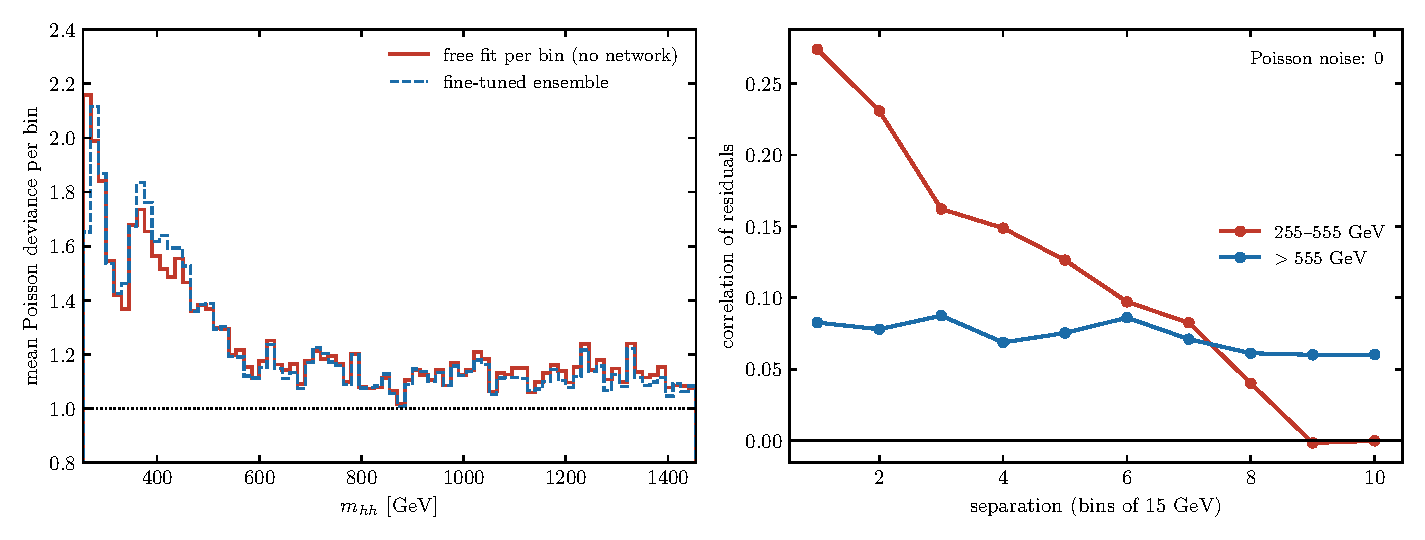
\includegraphics[width=\textwidth]{fig_floor.pdf}
\caption{Left: mean Poisson deviance per bin on the test spectra, for the free fit and the
ensemble; 1 is the value expected from Poisson noise alone. Right: correlation between the
residuals $z = (n - \hat n)/\sqrt{\hat n}$ of two bins of the same spectrum, as a function of
their separation. Poisson noise gives zero.}
\label{fig:floor}
\end{figure}

% ===========================================================================
\section{What the floor is}

\paragraph{Smooth deviations.} Poisson noise, and errors of the per-bin fit, are independent
from bin to bin. The residuals are not (\cref{fig:floor} right): below 555~GeV neighbouring
bins are correlated by 0.27, falling to zero over about 8 bins (120~GeV); above 555~GeV a
small correlation of about 0.07 persists at all separations. POWHEG departs from the 23-term
form by a smooth, spectrum-dependent amount.

\paragraph{Largest where the cross section cancels.} Define the cancellation ratio of a
spectrum as $\sigma_\text{tot}/\sum_k\sum_i|C_i a_{ik}|$: 1 when all terms add, small when the
cross section is a small difference of large terms. The excess depends strongly on it
(\cref{fig:cancel} left, \cref{tab:cancel}):

\begin{table}[h]
\centering
\small
\begin{tabular}{lccccc}
\toprule
cancellation quintile (1 = strongest) & 1 & 2 & 3 & 4 & 5 \\
\midrule
$\langle z^2\rangle$ (free fit, noise only) & 1.89 & 1.12 & 1.11 & 1.14 & 1.08 \\
lag-1 residual correlation, 255--555 GeV & 0.56 & 0.14 & 0.09 & 0.04 & 0.01 \\
lag-1 residual correlation, $>555$ GeV   & 0.24 & 0.05 & 0.05 & 0.02 & 0.01 \\
\bottomrule
\end{tabular}
\caption{Excess and smoothness of the residuals by degree of cancellation (200 test spectra
each).}
\label{tab:cancel}
\end{table}

The test spectrum with the strongest cancellation (815, ratio 0.0025: the cross section is
0.25\% of the sum of the magnitudes of its terms) is also the worst fitted, by the free fit and
the network alike, with a smooth shape that neither can follow (\cref{fig:cancel} right).
Where there is no cancellation, POWHEG agrees with the 23-term form almost to Poisson
precision.

\begin{figure}[h]
\centering
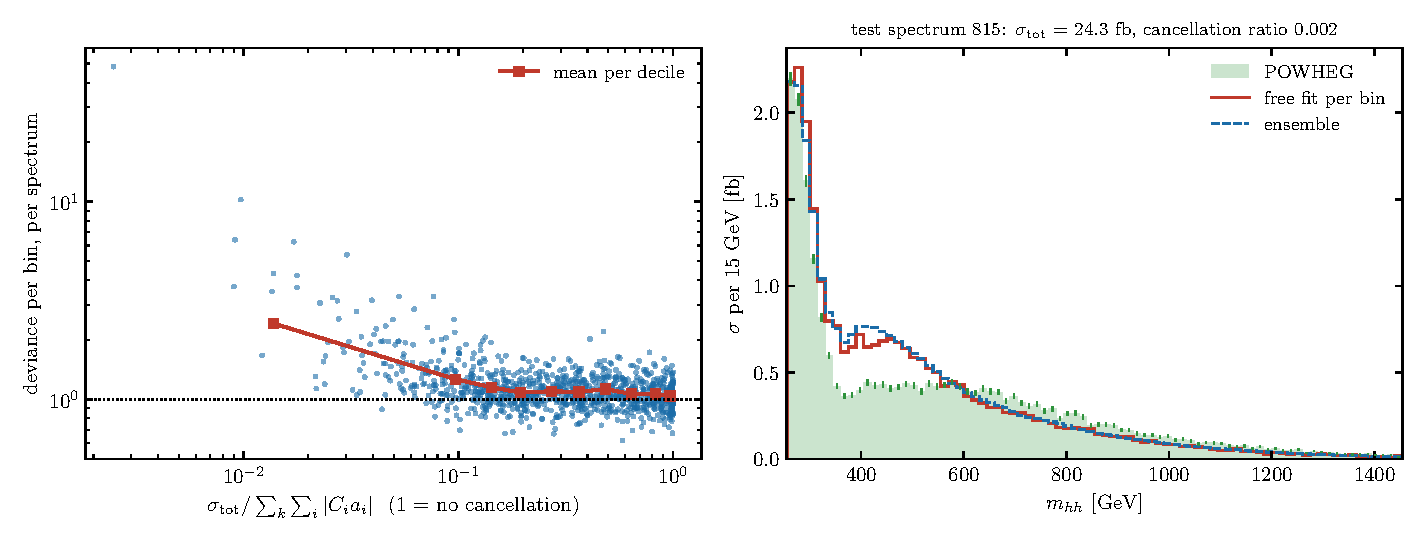
\includegraphics[width=\textwidth]{fig_cancel.pdf}
\caption{Left: mean deviance per bin of each test spectrum against its cancellation ratio;
squares: means in deciles. Right: the worst test spectrum (815), POWHEG with the free fit and
the ensemble.}
\label{fig:cancel}
\end{figure}

\begin{keyidea}[Interpretation]
A small \emph{relative} error on each of the 23 coupling components of the POWHEG cross
section, smooth in $m_{hh}$, is invisible when the components add, but is amplified when they
cancel: an error of 0.5\% on terms that cancel to 0.25\% of their size is a 200\% error on
the result. Such an error is a property of the samples, not of the network. Independent
noise, for example from negative-weight events, would not produce correlated residuals and is
disfavoured.
\end{keyidea}

% ===========================================================================
\section{A better model of the error}
\label{sec:better}

The interpretation suggests replacing the discrepancy term $a(m_{hh})\,\sigma_k^2$ by one
proportional to the size of the individual terms:
\begin{equation}
  s_\text{disc}^2 = \varepsilon(m_{hh})^2 \Big(\sum_{i=1}^{23} |C_i(\theta)\,a_i(m_{hh})|\Big)^2 .
\end{equation}
Fitted bin by bin on one half of the test spectra and checked on the other half (as a quick
test; for the paper it would be fitted on the quick-test rows):

\begin{table}[h]
\centering
\small
\begin{tabular}{lcccccccc}
\toprule
 & \multicolumn{3}{c}{$\langle z^2\rangle$} & \multicolumn{5}{c}{by cancellation quintile} \\
discrepancy & all & 255--555 & $>555$ & 1 & 2 & 3 & 4 & 5 \\
\midrule
$a(m_{hh})\,\sigma_k^2$ (current) & 1.054 & 1.157 & 1.019 & 1.52 & 0.95 & 0.95 & 0.95 & 0.90 \\
$\varepsilon(m_{hh})^2(\sum_i|C_ia_i|)^2$ & 1.013 & 1.043 & 1.003 & 0.98 & 0.97 & 1.04 & 1.06 & 1.02 \\
\bottomrule
\end{tabular}
\caption{Calibration of two discrepancy models on a held-out half of the test spectra, with
the free fit as the model.}
\label{tab:better}
\end{table}

The new form calibrates every degree of cancellation; the current one is too narrow for the
most cancelling spectra and slightly too wide for the rest. The fitted $\varepsilon$ is
0.1--0.2\% near threshold and up to about 0.9\% at higher $m_{hh}$: a plausible size for the
relative precision of a numerical calculation.

% ===========================================================================
\section{Plan}

\begin{enumerate}
  \item \textbf{Ask about the generator} (the colleague who produced the samples, and, if
    needed, the authors of the POWHEG \texttt{ggHH} implementation):
    \begin{itemize}
      \item How were the two-loop virtual amplitudes evaluated (interpolation grids, which
        version), and what is their quoted relative precision near threshold?
      \item Was each HEFT point an independent run with its own random seed and integration
        grids, or were spectra obtained by reweighting from a basis?
      \item Were negative-weight events produced, and how were they treated?
    \end{itemize}
    If a few spectra with strong cancellation could be regenerated with higher precision,
    a direct comparison would settle the origin.
  \item \textbf{Adopt the cancellation-aware discrepancy} for the paper: fit $\varepsilon(m_{hh})$
    on the quick-test rows with the Laplace mixture as the model, re-validate on the test
    spectra, and update the appendix, the figures and the summary.
  \item \textbf{Make the discrepancy smooth in $m_{hh}$}: a Gaussian-process term with
    amplitude $\varepsilon\sum_i|C_ia_i|$ and a correlation length fitted to the residuals
    (\cref{fig:floor} suggests 5--8 bins near threshold), in the spirit of Kennedy and O'Hagan.
    This is the principled version and matters for any use of the spectra that sums bins.
  \item \textbf{Keep the network.} The free fit shows nothing to gain in $\chi^2$. Remaining
    improvements to the model are about how well the individual $a_i$ are determined (the
    poorly constrained $a_{16}$--$a_{20}$), e.g.\ by fitting in a better-conditioned basis of
    the 23 monomials; they matter for interpreting the $a_i$, not for the cross section.
  \item \textbf{Keep the free fit as a benchmark} (\file{docs/modelerror/}) for any future
    change of model or data.
\end{enumerate}

\end{document}
